\documentclass[12pt,aspectratio=169]{beamer} %
\usetheme{CambridgeUS}
\usepackage{times}
\usepackage{tikz}
\usepackage{amsmath}
\usepackage{verbatim}
\usepackage{ctex}
\usepackage{booktabs}
\usepackage{ulem}
\usepackage{subcaption}
\usepackage{listings}
\lstset{escapeinside=``, breaklines=true, frame=none, extendedchars=false, basicstyle=\ttfamily, showstringspaces=false}
\usefonttheme{professionalfonts}
\usetikzlibrary{arrows,shapes,positioning}
\newcounter{cont}
\makeatletter
%allowframebreaks numbering in the title
\setbeamertemplate{frametitle continuation}{%
    \setcounter{cont}{\beamer@endpageofframe}%
    \addtocounter{cont}{1}%
    \addtocounter{cont}{-\beamer@startpageofframe}%
    (\insertcontinuationcount/\arabic{cont})%
}
\makeatother

\linespread{1.2}

% Background
\pgfdeclareimage[width=\paperwidth,height=\paperheight]{bg}{ecnu_background}
\setbeamertemplate{background}{\pgfuseimage{bg}}

\setbeamertemplate{frametitle}[default][left,leftskip=2cm]

\setbeamersize{text margin left=2cm,text margin right=2cm}

\catcode`\。=\active
\newcommand{。}{.}

\catcode`\,=\active
\newcommand{,}{, }

\catcode`\:=\active
\newcommand{:}{: }

\author[张羽戈 10165102136]{张羽戈 \\ 10165102136}
\date{2019 年 1 月 9 日}

\begin{document}

\title[Word Bubble]{基于单词模型的知识图谱构建 \\ Word Bubble}

% For every picture that defines or uses external nodes, you'll have to
% apply the 'remember picture' style. To avoid some typing, we'll apply
% the style to all pictures.
\tikzstyle{every picture}+=[remember picture]

% By default all math in TikZ nodes are set in inline mode. Change this to
% displaystyle so that we don't get small fractions.
\everymath{\displaystyle}

\begin{frame}
\titlepage % Print the title page as the first slide
\end{frame}

\begin{frame}
\frametitle{目标}
\begin{itemize}
\item 作业要求:知识图谱
\begin{itemize}
	\item 结点表示实体。
	\item 实体与实体之间的关系。
	\item 在已有关系的基础上实现「推理」。
\end{itemize}
\item 具体任务
\begin{itemize}
	\item 找一个合适的领域。
	\item 搜集这个领域中的实体和实体之间的关系数据。
	\item 建立一套查询系统 (比如 Cypher)。
	\item 将查询结果展示出来 (比如 Neo4j Browser)。
\end{itemize}
\end{itemize}

\end{frame}

\begin{frame}
\frametitle{想法}
\begin{itemize}
\item 实体:英文单词。
\item 关系:英文单词之间的天然的关系。
\begin{itemize}
	\item 同义词。
	\item 紧密相关的词。
	\item 词组搭配 (葡萄配红酒)。
	\item 词根 (Word Family)。
\end{itemize}
\item 查询:
\begin{itemize}
	\item 一个单词的近邻。有用!
	\item 两个单词的距离。无用!
\end{itemize}
\end{itemize}
\end{frame}

\begin{frame}
\frametitle{数据准备}
\begin{itemize}
\item 开始:
\begin{itemize}
	\item 牛津 3000 核心词汇表 (3839)。
	\item 学术单词表 (AWL 10 Sublists)。
\end{itemize}
\item 爬取 Macmillan Dictionary。
\begin{itemize}
	\item 省下了 API 昂贵的开销。
\end{itemize}
\item 用网页中的单词链接加深搜索。
\item 两次迭代:14801 词条,8576 词组,3157 索引 (同义词 + 相关词)。
\item 使用 py2neo 将数据注入到 Neo4j。
\end{itemize}
\end{frame}

\begin{frame}
\frametitle{一些数据:度数最多的点}

\texttt{match (k:Word) with k, size((k)--()) as degree where degree > 30 return k.name, degree}

\vspace*{12pt}

\begin{center}
\begin{tabular}{cc}
\toprule
Word & Degree \\
\midrule
get & 165 \\
put & 115 \\
around & 69 \\
day & 60 \\
\bottomrule
\end{tabular}
\end{center}

\end{frame}

\begin{frame}
\frametitle{一些数据:连通性}

\texttt{match (u) return u.partition as partition, count(*) as size order by size desc}

\vspace*{12pt}

\begin{center}
\bf
CONNECTED!
\end{center}

\end{frame}

\begin{frame}
\frametitle{一些数据:最长最短路}

\begin{itemize}
\item 需要求所有点对最短路,使用 C++ 实现。
\item 最大距离为 18。
\end{itemize}

\vspace*{12pt}

\begin{center}
\begin{tabular}{cc}
\toprule
Source & Target \\
\midrule
Monday & disdain \\
Monday & fake \\
Monday & hypothesize \\
\bottomrule
\end{tabular}
\end{center}

\end{frame}


\begin{frame}
\frametitle{实体设计}
\begin{itemize}
\item 单词 (具体词性)。
\begin{itemize}
	\item Id, Name, Group, Part 以属性存储。Senses 以 JSON 存储。
	\item 保留所有例句中的链接,方便跳转。
	\item 剔除空词条、无法处理的释义等。
\end{itemize}
\item 抽象词条 (抽象词性):没有具体的页面对应。
\item 词组:带空格的都算。
\item 索引。
\end{itemize}
\end{frame}


\begin{frame}
\frametitle{查询设计}
\begin{itemize}
\item 使用 Javascript 调用 Neo4j REST API。
\item 查询一个单词若干跳内的邻居。
\begin{itemize}
	\item 太多怎么办:停用词处理。
	\item 找不到怎么办:警告信息。
	\item 实体查询方法:默认以 Name 查询,可以指定字段 \\ $\rightarrow$ \textbf{翻译成 Cypher}。
	\item 用户不会写怎么办:跳转链接 (交互设计)。
\end{itemize}
\item 查询两个单词之间的路径。
\end{itemize}
\end{frame}


\begin{frame}[allowframebreaks]
\frametitle{难点:可视化与交互设计}
\begin{itemize}
\item 不使用 Neo4j Browser:
\begin{itemize}
	\item 没办法自定义。
	\item 不开源,无法嵌入。
	\item 与查询联动较差。
\end{itemize}
\item 实现本地应用:Electron.js。
\item 使用 Material UI:React + Material-UI。
\item 可视化类库:d3.js。
\end{itemize}

\framebreak

\begin{itemize}
\item 模块:
\begin{itemize}
	\item 搜索框 (SearchBar)。
	\item 结点关系图 (Graph)。
	\item 最佳匹配词条 (Entry)。
\end{itemize}
\item 联动:
\begin{itemize}
	\item SearchBar $\leftrightarrow$ Graph.
	\item SearchBar $\leftrightarrow$ Entry.
	\item Graph $\leftrightarrow$ Entry.
\end{itemize}
\end{itemize}

\framebreak

\begin{itemize}
\item 搜索框细节:
\begin{itemize}
	\item 搜索历史回溯。
	\item 从上一次到这一次走了有多远。
\end{itemize}
\item 词条内容:
\begin{itemize}
	\item 看起来不比词典差。
\end{itemize}
\end{itemize}

\framebreak

\begin{itemize}
\item 图的实现:
\begin{itemize}
	\item 带碰撞检测的力导向图。
	\item 词条的自动字体大小和自动换行设计。
	\item 可自定义的类别颜色区分和类别隐藏。
	\item 可自定义的自动缩放。
\end{itemize}
\item 痛点:在 React 上用 d3,DOM 操作无法回避,且新增同步问题。
\end{itemize}

\end{frame}

\begin{frame}
\begin{center}

\includegraphics[height=0.8\paperheight]{showtime.png}
\end{center}
\end{frame}


\begin{frame}[allowframebreaks]
\frametitle{比较:Visuwords}

\begin{center}
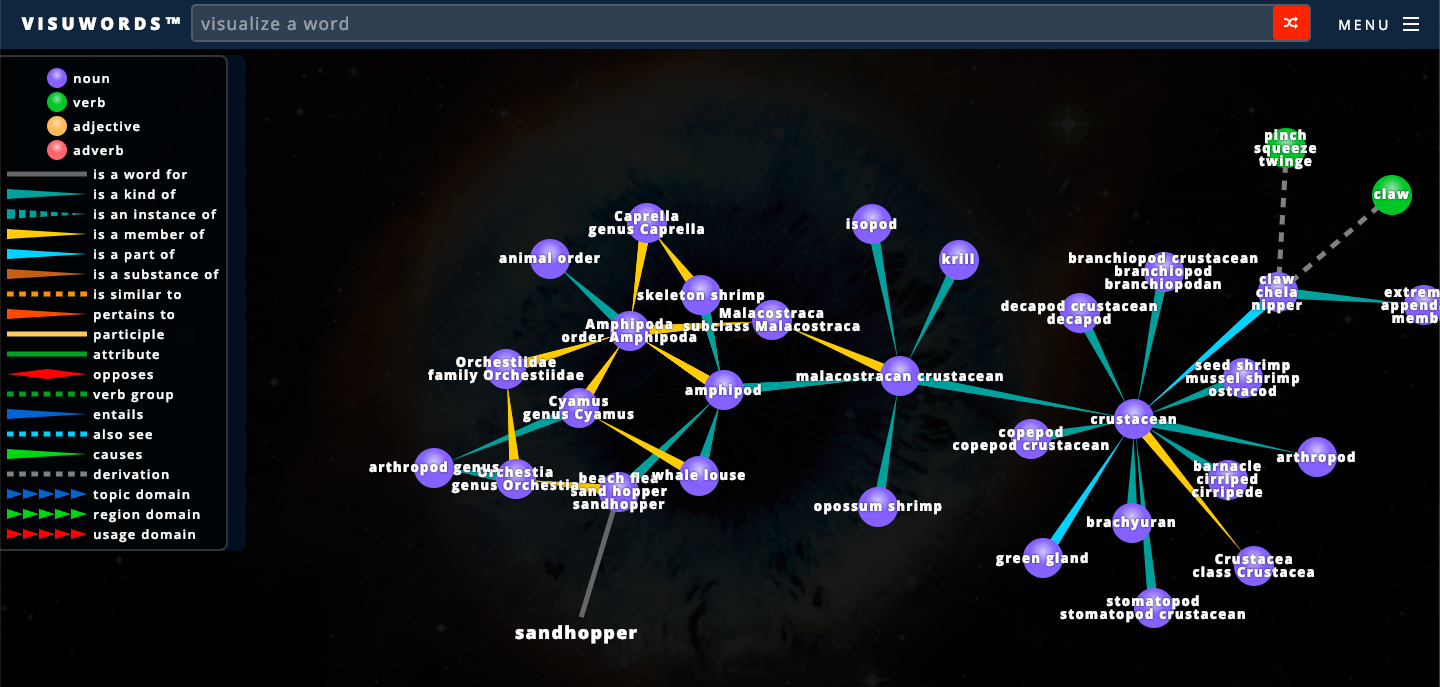
\includegraphics[width=\linewidth]{visuwords.png}
\end{center}

\framebreak

\begin{itemize}
\item 优点:
\begin{itemize}
	\item 图支持增量扩充。
	\item 支持的关系种类多,区分明确。
\end{itemize}
\item 缺点:
\begin{itemize}
	\item 丑。
	\item 没有「词典」的功能。
\end{itemize}
\end{itemize}

\end{frame}


\begin{frame}[allowframebreaks]
\frametitle{比较:Visual Thesaurus}

\begin{center}
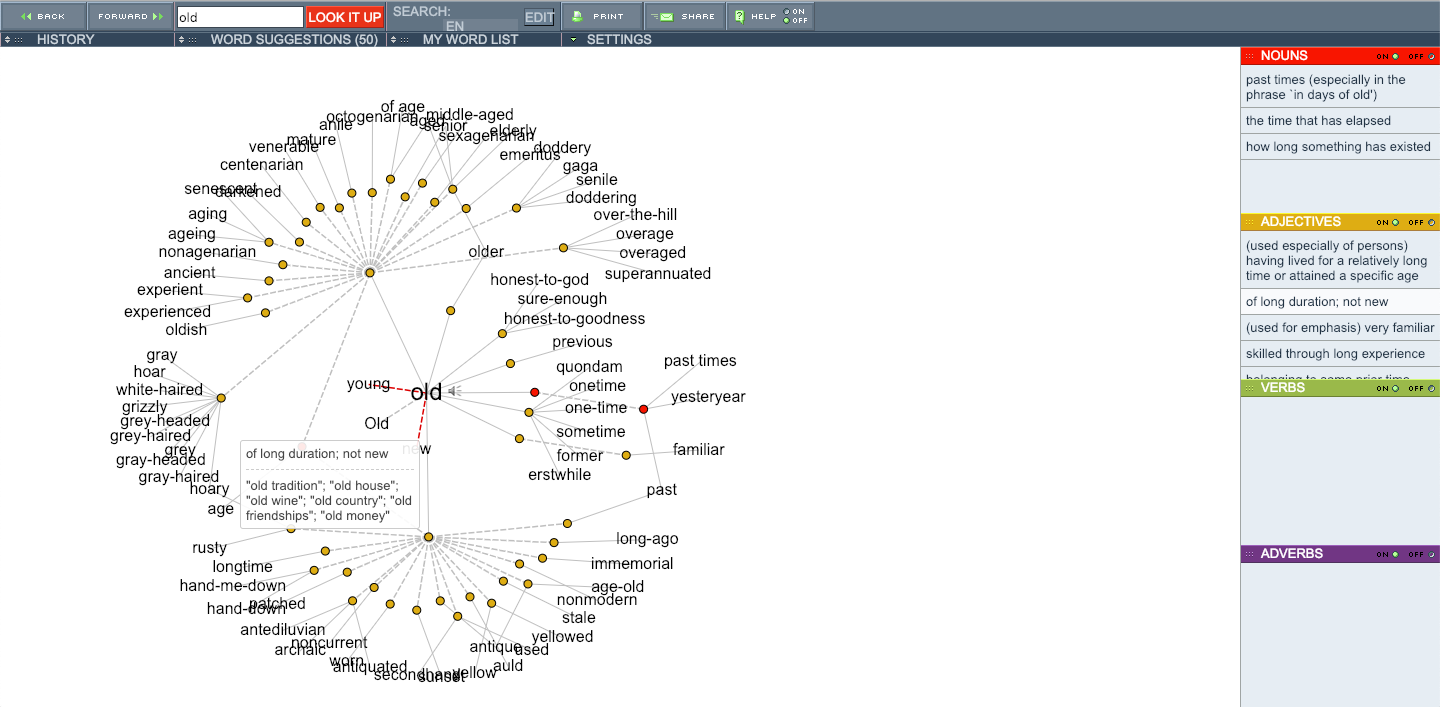
\includegraphics[width=\linewidth]{visualthesaurus.png}
\end{center}

\framebreak

\begin{itemize}
\item 优点:
\begin{itemize}
	\item 释义分开列举,有交互。
	\item 历史、提示功能强大。
\end{itemize}
\item 缺点:
\begin{itemize}
	\item 界面复古。
	\item 付费。
\end{itemize}
\end{itemize}

\end{frame}



\begin{frame}[allowframebreaks]
\frametitle{比较:ConceptNet}

\begin{center}
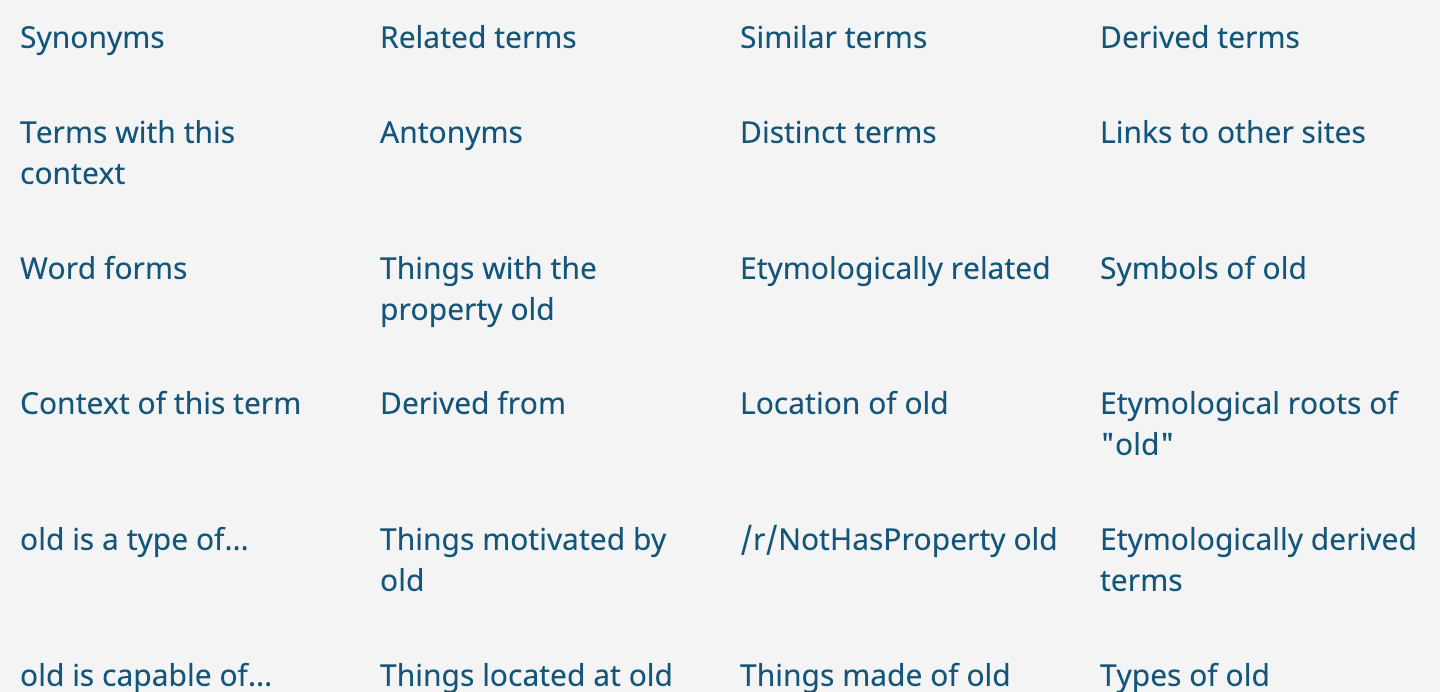
\includegraphics[width=\linewidth]{conceptnet.png}
\end{center}

\framebreak

\begin{itemize}
\item 优点:
\begin{itemize}
	\item 关系种类非常丰富。
	\item 历史悠久的开源软件,拥有上千 star。
\end{itemize}
\item 缺点:
\begin{itemize}
	\item 原生可视化支持较弱(不支持?)。
\end{itemize}
\end{itemize}

\end{frame}

\begin{frame}

\frametitle{说到开源,我就想到……}

\begin{itemize}
\item Word Bubble 会在结课后开源。

\begin{center}
\url{https://github.com/ultmaster/}
\end{center}

\item 希望大家多多关注。
\end{itemize}

\end{frame}



\end{document}
              